\section{Limits}

\subsection{Delta-Epsilon Definition on R}

The limit of $f$ as $x$ approaches $a$ is $L$ if given a positive real number
$\epsilon$, there exists a corresponding $\delta$ so that numbers selected with distance from $a$
less than $\delta$ and $>0$ it is guaranteed that outputs under $f$ are within distance $\epsilon$ from $L$.

Formal definition:

$\lim_{x\to a}f(x)=L$ if $\forall \epsilon >0$, $\exists\delta > 0$ such that $0< |x-a| < \delta \implies |f(x)-L|<\epsilon$

\subsection{Definition of Limit on R2}

If $f:\R^2\to \R$ and $P_0=(x_0,y_0)$, then $\lim _{(x, y) \rightarrow\left(x_{0}, y_{0}\right)} f(x, y)=L$ 
if given any small positive number $\epsilon$, $\delta>0$ is guaranteed so when there is a point $C\neq P_0$ within circle of radius $\delta$ about $P_0$, $f(x,y)$ lies within $\epsilon$ of $L$.

Formally: 

\[\lim _{(x, y) \rightarrow\left(x_{0}, y_{0}\right)} f(x, y)=\lim _{\tb{x} \rightarrow P_{0}} f(x, y)=L \text { if } \forall \varepsilon>0 \;\exists \delta>0\]

such that

\[0<\sqrt{\left(x-x_{0}\right)^{2}+\left(y-y_{0}\right)^{2}}<\delta \Longrightarrow|f(x, y)-L|<\varepsilon\]

\subsection{Continuous Functions}

\begin{itemize}
    \item Polynomials: $f(x,y)=x^2y+xy^2$
    \item Exponentials: $f(x,y)=e^{xy}$
    \item Trigonometric: $f(x,y)=\sin(x+y)$
    \item Compositions of any continuous functions: $f(x,y)=\cos(e^{x^2y-xy^2})$
    \item Sums, differences, products of continuous functions: $f(x, y)=x^{2} y-x y^{2}+e^{x y} \sin (x y)$
    \item Quotients of continuous functions (domain of quotient does not include zeros of denominator): $f(x, y)=\frac{x^{2 y}-x y^{2}}{\sin (x y)}$
\end{itemize}

\subsection{Computational Techniques}

Can use continuity to find limit (plug in point). Can also use conjugate multiplication to simplify and compute. Cancelling terms works because a limit approaches a value instead of equaling it.
Can also squeeze a function between 2 continuous ones to find limit.

Let $\lim _{(x, y) \rightarrow(0,0)} \frac{x^{2}}{\sqrt{x^{2}+y^{2}}}$ exist.
Know that $0\leq \lim _{(x, y) \rightarrow(0,0)} \frac{x^{2}}{\sqrt{x^{2}+y^{2}}}$.
Because $y^2>0$, $\frac{x^{2}}{\sqrt{x^{2}+y^{2}}} \leq \frac{x^{2}+y^{2}}{\sqrt{x^{2}+y^{2}}}$.
Thus, $\lim _{(x, y) \rightarrow(0,0)} 0 \leq \lim _{(x, y) \rightarrow(0,0)} \frac{x^{2}}{\sqrt{x^{2}+y^{2}}} \leq \lim _{(x, y) \rightarrow(0,0)}\left(x^{2}+y^{2}\right)^{1 / 2}$
so the limit is 0.

Other strategies: If a term $k(x,y)\geq 0\;\forall\; (x,y)\in \R^2$, then can simply perform $\pm 1$ to denominator for squeeze theorem proofs.

\subsection{Common inequalities and proofs}

\begin{itemize}
    \item AM-GM inequality: $\frac{x+y}{2}\geq \sqrt{xy}\implies (x-y)^2\geq 0$
    \item Triangle inequality: $|x+y|\leq |x|+|y|$ and $|x-y|\geq |x|-|y|$
    \item $|e^x-1|\leq |x|e^{|x|}$
\end{itemize}

Proof that $\frac{\sin x}{x}=1$:

\begin{center}
    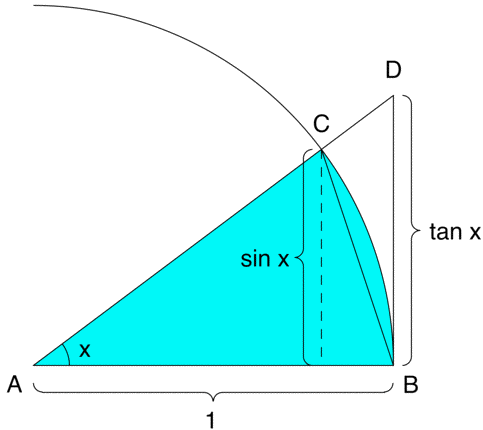
\includegraphics[scale=0.4]{Screen Shot 2021-04-21 at 10.59.12 AM.png}
\end{center}

It is evident that:
\begin{gather}
    \frac{1}{2}\sin x\leq \frac{1}{2}x\leq \frac{1}{2}\tan x\\
    \sin x\leq x \leq \tan x\\
    1\leq \frac{x}{\sin x}\leq \frac{1}{\cos x}\\
    1\geq \frac{\sin x}{x}\geq \cos x
\end{gather}

Applying the squeeze theorem to 4:

\begin{gather*}
    \lim_{x\to 0}1\geq \lim_{x\to 0}\frac{\sin x}{x}\geq \lim_{x\to 0} \cos x\\
    1\geq \frac{\sin x}{x}\geq 1
\end{gather*}

Thus, $\lim_{x\to 0}\frac{\sin x}{x}=1$.

\section{Derivatives}

\subsection{Limit Definition}

A function $f:\R^m \to \R^n$ is differentiable at $P_0$ if there is a linear transformation from $n\times m$ matrix $Df(P_0)$ satisfying

\[\lim_{\tb{x}\to P_0}\frac{\big\vert \big\vert f \big( \tb{x} \big)-\big(f(P_0)+\mathrm{D}f(P_0)(\tb{x}-P_0) \big) \big\vert \big\vert}{\vert \vert \tb{x}-P_0 \vert \vert}=0\]

If the function is differentiable at this point, then $Df(P_0)$ is the derivative of $f$ at $P_0$. Called Jacobian matrix of $f$ at $P_0$.

Can adapt this to single-variable calculus:

\[\displaystyle \lim_{x\to a} \frac{\vert f(x)-\big(f(a)+(m_a)(x-a)\big) \vert}{\vert x-a \vert}=0\]

Simplifying and reconfiguring to limit definition of a derivative:

\begin{align*}
    \lim_{x\to a} \frac{\vert f(x)-\big(f(a)+(m_a)(x-a)\big) \vert}{\vert x-a \vert}&=0\\
    \lim_{x\to a}\left\vert \frac{f(x)-\big(f(a)+(m_a)(x-a)\big)}{x-a} \right\vert&=0\\
    \left \vert \lim_{x\to a} \frac{f(x)-\big(f(a)+(m_a)(x-a)\big)}{x-a} \right \vert&=0\\
    \lim_{x\to a} \frac{f(x)-\big(f(a)+(m_a)(x-a)\big)}{x-a}&=0 \, \mbox{since}\, \vert 0 \vert=0\\ 
    \lim_{x\to a} \left( \frac{f(x)-f(a)}{x-a}-m_a\right)&=0\\
    \lim_{x\to a}\frac{f(x)-f(a)}{x-a}&=m_a
\end{align*}

Equivalent to the case of a $1\times 1$ matrix $Df(P_0)$ where the single entry is $f'(a)$.
Also $m_a=f'(a)\implies f(x)=f(a)+f'(a)(x-a)$ is the linear approximation. 

As $x$-values approach $a$, $f(x)-(f(a)+f'(a)(x-a))$ approaches 0 faster. Thus, $\frac{f(x)-\big(f(a)+f'(a)(x-a)\big)}{x-a}$ approaches 0.

\subsection{Multivariable Application}

Approximating plane of some $f:\R^2\to \R$ is $L_{P_0}(x,y)=f(a,b)+f_x(a,b)(x-a)+f_y(a,b)(y-b)$, i.e. the plane spanned by
$\langle 1,0,f_x(a,b)\rangle$ and $\langle 0,1,f_y(a,b)\rangle$ passing through $(a,b,f(a,b))$.

Is identical to $\begin{bmatrix}f_x(P_0)&f_y(P_0)\end{bmatrix}\begin{bmatrix}x-a\\y-b\end{bmatrix}$. The matrix is the matrix of partial derivatives.

Such a function is differentiable if:

\[\displaystyle \lim_{(x,y)\to(a,b)}\frac{f(x,y)-\left(f(a,b)+\Big(\begin{matrix} f_x(a,b)&f_y(a,b) \end{matrix} \Big)\left(\begin{matrix}x-a\\y-b\\ \end{matrix} \right) \right)}{\sqrt{(x-a)^2+(y-b)^2}}=0\]

Numerator is linear approximation and denominator is distance to point $(a,b)$. Thus:

\[\boxed{f(x,y) \mbox{ is differentiable at the point }P_0\mbox{ if}\displaystyle \lim_{(x,y)\to P_0}\frac{|f(x,y)-L_{P_0}(x,y)|}{||(x,y)-P_0||}=0}\]

Geometrically, if a circle about $P_0$ is drawn and radius is collapsed, distance between $f$ and approximating plane will become 0 much faster, so fraction becomes 0.

If there is a radius $\delta > 0$ on the disk of radius $\delta$ centered at $P_0$, $f_x(x,y)$ and $f_y(x,y)$ are continuous at every point on the disk, then $f(x,y)$ is continuous at every point on the disk.
Differentiability can not be established by the existence of partial derivatives at a point, it is sufficient to demonstrate continuous partials
at a point.

The criteria for differentiability are that $f_x,f_y$ exist and $f$ is locally linear at $P_0$. The tangent plane exists here. However,
it is sufficient to demonstrate differentiability by showing that both $f_x$ and $f_y$ are continuous on an open disk $D$ to conclude that $f(x,y)$
is differentiable on $D$. Alternatively, the above limit definition can be used.

If a function $f:\R^m\to \R^n$ exists, then it is made up of $n$ component functions on $\R^m$. The Jacobian matrix is as follows:

\[Df\left( x_1,\ldots x_m\right) =\begin{bmatrix} \nabla f_{1}\left(x_1,\ldots x_m\right) \\ \vdots \\ \nabla f_{n}\left(x_1,\ldots x_m\right) \end{bmatrix}\]

The number of rows $n$ depends on components (codomain) of the output space whereas the domain determines columns ($m$). Thus, linear approximation to a function $f:\R^m\to \R^n$ at $P_0$ is

\[L_{P_0}(\tb{x})=f(P_0)+\Big(\mbox{matrix of partial derivatives at}\,P_0\Big)(\tb{x}-P_0)\]

In parametric equations (paths), let $\tb{c}(t)=\big(x(t), y(t), z(t) \big)$ have continuous partials.
Thus, the matrix of partials $D\tb c(t)=\begin{bmatrix}x'(t)\\y'(t)\\z'(t)\end{bmatrix}$. Is the vertical velocity vector.
If the approximation $L_{t_0}(t)$ is found, it yields:

\begin{align*}
    L_{t_0}(t)&=\tb c(t_0)+
    \left(
    \begin{matrix}
    x'(t_0)\\
    y'(t_0)\\
    z'(t_0)\\
    \end{matrix}
    \right)
    (t-t_0)\\
    &=\tb{c} (t_0)+(t-t_0)\tb c\,'(t_0)
\end{align*}

Also, note that matrix of partials for a scalar valued function $f:\R^n\to \R$ is simply the gradient; there is 1 row and $n$ columns in the gradient vector.

\section{Derivative Rules}

\subsection{Fundamental Rules}

If $f,g:\R^m\to \R^n$ are differentiable at $P_0\in \R^m$ for $c\in \R$:
\begin{itemize}
    \item $h(\tb{x})=cf(\tb{x})\implies \mathrm{D}h(P_0)=cDf(P_0)$
    \item $h(\tb{x})=f(\tb{x})+g(\tb{x})\implies \mathrm{D}h(P_0)=\mathrm{D}f(P_0)+\mathrm{D}g(P_0)$ (domain = codomain; sum of two $n\times m$ matrices)
\end{itemize}

If $f,g:\R^n\to \R$ are differentiable at $P_0\in \R^n$:
\begin{itemize}
    \item $h(\tb{x})=f(\tb{x})g(\tb{x})\implies \mathrm{D}h(P_0)=f(P_0)\mathrm{D}g(P_0)+g(P_0)\mathrm{D}f(P_0)$ (no commutativity as matrix times scalar DNE)
\end{itemize}

If $f,g:\R^n\to \R$ are both differentiable at $P_0\in \R^n$ and $g(P_0)\neq 0$:
\begin{itemize}
    \item $\mathrm{D}\left(\frac{f}{g}\right)(P_0)=\frac{g(P_0)\mathrm{D}f(P_0)-f(P_0)\mathrm{D}g(P_0)}{g(P_0)^2}$
\end{itemize}

\subsection{Chain Rule}

If $g:\R^m\to \R^p$ and $f:\R^p\to \R^n$ and $g$ is differentiable at $P_0\in \R^m$ and the same for $f$ at $g(P_0)$:
\begin{itemize}
    \item $\mathrm{D}\Big(f\circ g\Big)(P_0)=\mathrm{D}f\big(g(P_0)\big)\mathrm{D}g(P_0)$
\end{itemize}

Thus, derivative of composites is a matrix product. $\mathrm{D}f(g(P_0))\to n\times p$ and $\mathrm{D}g(P_0)\to p\times m$
so $\mathrm{D}(f\circ g)(P_0)\to n\times m$.

If $\tb{c}:\R\to \R^n$ is a path differentiable at $t_0\in \R$ and $f:\R^n\to \R$ is differentiable at $\tb{c}(t_0)$, then:

\[\frac{d}{dt}f(\tb{c}(t_0))=\mathrm{D}f(\tb{c}(t_0))D\tb{c}(t_0)=\left[ \nabla f\left( x_{1},x_{2},\ldots x_{n}\right) \right]\begin{bmatrix} \vdots \\ \tb{c}\,'(t_0) \\ \vdots \end{bmatrix}=\nabla f(\tb{c}\,'(t_0))\cdot \tb{c}\,'(t_0)\]

Thus, derivative of scalar valued function and path is dot product of gradient and velocity.

\section{Gradient}

\subsection{Directional Derivative}

Directional derivative of a scalar function $f:\R^n\to \R$ at some $P_0\in\R^n$ in the direction of $\tb{v}\in\R^n$ is given by

\[\boxed{f_{\tb{v}}\left(P_{0}\right)=\nabla f\left(P_{0}\right) \cdot \frac{\tb{v}}{\|\tb{v}\|}}\]

Maximizing the directional derivative involves the dot product. Let $f:\R^n\to \R$ and $P_0\in\R^n$ where $\nabla f(P_0)$ is defined.
Also, let $\tb{u}$ be a unit vector such that $f_{\tb{u}}(P_0)$ is maximized. The directional derivative is

\[f_{\tb u}(P_0)=\nabla f(P_0)\cdot \tb u=\|\nabla f(P_0)\|\cos \theta\]

Since $\cos\theta \in [-1,1]$, the directional derivative is maximized at $\cos\theta = 1\implies \tb{u}||\nabla f(P_0)||$.
\textbf{Thus the gradient of a function at $P_0$ points in the direction of steepest ascent}.

For a more general case given $f:\R^n\to \R$ and $P_0\in\R^n$ where $\nabla f_{\tb{v}}(P_0)$ is maximized and $\nabla f(P_0)$ exists:
\begin{align*}
    \nabla f_{\tb{v}}(P_0)&=\nabla f(P_0) \cdot \frac{\tb{v}}{||\tb{v}||}\\
    &=\nabla f(P_0) \cdot \frac{\nabla f(P_0)}{||\nabla f(P_0)||}\\
    &=\frac{\nabla f(P_0)\cdot \nabla f(P_0)}{||\nabla f(P_0)||}\\
    &=||\nabla f(P_0)||
\end{align*}

Thus, the length of the gradient vector tells how steep the ascent is in the direction of the steepest ascent.

\subsection{Gradient Fields}

A image in the codomain $\R^n$ where arrows originating at each point point in the steepest direction $\forall\; P\in \R^n$ where the partials exist.
Are always perpendicular to level curves of $f$.

Let $f:\R^n\to \R$ and $P\in \R^n$ a point where partials of $f$ exist. Considering the level set $f(\tb{x})=f(P)$,
all values map to same codomain value as $P$. Also, let $\tb{c}:\R^n\to \R$ have an image entirely within this level set $f(\tb{x})=f(P)$
and $\tb{c}(t_0)=P$. Then, the proof must show that $\nabla f(P)\cdot \tb c\,'(t_0)=0$.

Note that since $h(t)=f(\tb{c}(t))$, $h'(t_0)=\nabla f \Big(\tb c (t_0) \Big)\cdot \tb c\,'(t_0)=\nabla f (P)\cdot  \tb c\,'(t_0)$.
Since the image of $\tb{c}(t)$ lies within $f(\tb{x})=f(P)$, $f$ is constant on the image of $\tb{c}$ (every point on $\tb{c}$ maps to $f(P)$ under $f$).
Thus, $h(t)=f(\tb{c}(t))\implies h'(t)=0\;\forall\;t$.

\subsection{Sphere}

Sphere is not a function as a point $P=(x,y)$ correspond to multiple $z$ values.
Can be viewed as a level surface in $\R^3$ for some $f:\R^3\to \R$. The function is $f(x,y,z)=x^2+y^2+z^2$
and the level surface sphere is $x^2+y^2+z^2=R^2$ where $R$ is the radius.
Given the point $(0,0,R)$, the gradient is upward along the $z$-axis. All curves passing through this point
have a tangent vector perpendicular to $\nabla f(0,0,R)$ since gradients are perpendicular to level sets.
It can be said that any vector perpendicular to $\nabla f(0,0,R)$ is a tangent to at least 1 curve in the sphere passing through $(0,0,R)$.
Thus, the perpendicular space to $\nabla f(0,0,R)$ forms a plane of tangent vectors at $(0,0,R)$ and is a tangent plane.
An expression for the tangent plane is 

\begin{align*}
    \nabla f (0,0,R)\cdot(x-0, y-0, z-R)&=0\\
    f_x(0,0,R)x+f_y(0,0,R)y+f_z(0,0,R)&=0\\
    2(0)x+2(0)y+2(R)(z-R)&=0\\
    2Rz-2R^2&=0\\
    z&=R\\
\end{align*}

Expression for the tangent plane to a level set of some $f:\R^3\to \R$:

\begin{align*}
    \nabla f (P_0)\cdot(x-x_0, y-y_0,z- z_0)&=0\\
    f_x(P_0)(x-x_0)+f_y(P_0)(y-y_0)+f_z(P_0)(z-z_0)&=0\\
    f_x(P_0)x+f_y(P_0)y+f_z(P_0)z&=\nabla f(P_0)\cdot P_0\\
\end{align*}
$$\boxed{f_x(P_0)x+f_y(P_0)y+f_z(P_0)z=\nabla f(P_0)\cdot P_0}$$

\section{Implicit Function Theorem}

\subsection{Single variable}

Is the explanation behind single-variable implicit differentiation.

If $F:\R^2\to \R$ is of class $C^1$ and there is a point $\tb{x}_0=(a,b)\in\R^2$ such that 
$F(a,b)=0$ and $F_y(a,b)\neq 0$, then it is guaranteed that
\begin{itemize}
    \item There is some small $\delta>0$ and some small $\epsilon>0$ so that for $(x,y)\in\R^2$ with $|x-a|<\delta$ and $|y-b|<\epsilon$ there is a unique function $g:\R\to\R$ satisfying
    $F(x,g(x))=0$ and any point on the level set $F(x,y)=0$ satisfying these 2 conditions on coordinates will have property $y=g(x)$. To summarize, near the point $(a,b)$ points on $F(x,y)=0$ lie on the graph of a unique function $y=g(x)$.
    \item $g$ is of class $C^1$; differentiable so $g'(x)$ is continuous and $g'(x)=-\frac{F_x}{F_y}$
\end{itemize}

\subsection{Multivariable definition}

If $F:\R^2\to \R$ is of class $C^1$ and there exists $\tb{x}_0=(a,b,c)\in\R^3$ such that
$F(a,b,c)=0$ and $F_z(a,b,c)\neq 0$ then is is guaranteed that
\begin{itemize}
    \item There is some small $\delta > 0$ and $\epsilon > 0$ so that for $(x,y,z)\in\R^3$ with $\sqrt{(x-a)^2+(y-b)^2}<\delta$ and $|z-c|<\epsilon$ there is a unique function $g:\R^2\to\R$
    that satisfies $F(x,y,g(x,y))=0$ and any point satisfying these inequalities on $x,y,z$-coordinates that lies on $F(x,y,z)=0$ will have the property $z=g(x,y)$, so near the point $(a,b,c)$ on the level set $F(x,y,z)=0$ points can be seen as lying on $z=g(x,y)$.
    \item $g$ is of class $C^1$ so it is differentiable and both partials exist and are continuous, and $g_x(x,y)=-\frac{F_x}{F_z},g_y(x,y)=-\frac{F_y}{F_z}$.
\end{itemize}

The IFT can justify the existence of a tangent plane to a surface.

Let $F:\R^3\to \R$ be of class $C^1$ and the surface $S=\{(x,y,z)\in\R\;|\;F(x,y,z)=c\}$ for some $c\in\R$ be the level set of $F$.
The tangent plane is given by $F_x(P)x+F_y(P)y+F_z(P)z=\nabla F(P)\cdot \tb P$ for $P=(x_0,y_0,z_0)$. The plane is not defined when
$\nabla F(P)=\tb 0$. 

Applying the IFT, this plane is tangent to $S$. If $\nabla F(P)\neq \tb 0$ then at least one of $F_x,F_y,F_z\neq 0$ at $P$.
Without loss of generality, let $F_z\neq 0$. Then, let $f(x,y,z)=F(x,y,z)-c$. Since $f_z(P)=F_z(P)\neq 0$, applying the IFT to $f$ makes the conclusion that 
near $P$ $z$ is a differentiable function of $x,y$ so that there is a unique function $g:\R^2\to \R$ such that $z=g(x,y)$. The tangent plane to $g$ at $P$ is 
\begin{align*}
    z &=g\left(x_{0}, y_{0}\right)+g_{x}\left(x_{0}, y_{0}\right)\left(x-x_{0}\right)+g_{y}\left(x_{0}, y_{0}\right)\left(y-y_{0}\right) \\
    &=z_{0}+g_{x}\left(x_{0}, y_{0}\right)\left(x-x_{0}\right)+g_{v}\left(x_{0}, y_{0}\right)\left(y-y_{0}\right)
\end{align*}

It can then be shown that this plane is the same as given by the gradient approximation:

It follows that $f_x(P)=F_x(P)$ and $f_y(P)=F_y(P)$. Then,

\begin{align*}
    z&=z_0+g_x(x_0,y_0)(x-x_0)+g_y(x_0,y_0)(y-y_0)\\
    z&=z_0-\frac{F_x(P)}{F_z(P)}(x-x_0)-\frac{F_y(P)}{F_z(P)}(y-y_0)\\
    F_z(P)z&=F_z(P)z_0-F_x(P)x+F_x(P)x_0-F_y(P)y+F_yy_0\\
    F_x(P)x+F_y(P)y+F_z(P)z&=F_z(P)z_0+F_x(P)x_0+F_y(P)y_0\\
    F_x(P)x+F_y(P)y+F_z(P)z&=\nabla F(P)\cdot P
\end{align*}

\subsection{IFT for vector-valued functions}

Let $F:\R^{m+n}\to \R^n$ be of class $C^1$, then 
\[F(x_1, x_2, x_3,...,x_m, z_1, z_2, ..., z_n)=\Big(F_1(\mbox{input vector}), F_2(\mbox{input vector}), F_3(\mbox{input vector}),...,F_n(\mbox{input vector})\Big)\]

The inputs to $F$ are the $m$-dimensional vector $\tb x_0=(x_1,x_2,\ldots,x_m)$ and the $n$-dimensional vector $\tb z_0=(z_1,z_2,\ldots, z_n)$.
The conditions for IFT are met when
\begin{itemize}
    \item $F(\tb x_0)=\tb 0$
    \item $\mbox{Det}\left(
        \begin{matrix}
        \frac{\partial F_1}{\partial z_1}&\dots&\frac{\partial F_1}{\partial z_n}\\
        \vdots&\ddots&\vdots\\
        \frac{\partial F_n}{\partial z_1}&\dots&\frac{\partial F_n}{\partial z_n}
        \end{matrix}
        \right)\neq 0$
\end{itemize}

Then there is a unique $C^1$ function $g:\R^m\to \R^n$ such that for all points satisfying $F(\tb v)=\tb 0$ that are sufficiently near $P=(\tb x_0,\tb z_0)$ we can conclude $\tb z=g(\tb x)$. Lastly,
\[\boxed{\textbf{A $C^1$ function is locally invertible where its derivative is}}\]

This is reasonable because a linear approximation acts in an invertible way locally, so both the derivative and function can be said to be invertible.

\subsection{Example problem}

Given a nonlinear system of equations:
\begin{align*}
    xu+yvu^2&=2\\
    xu^3+y^2v^4&=2\\
\end{align*}

Implicit differentiation is done by treating $u$ and $v$ as functions of $x,y$. In this case,
can find how a small change in $x$ affects $u$ when all variables are 1 (i.e. $(x,y,u,v)=(1,1,1,1)$)).
First equation differentiation gives 

\begin{align*}
    \frac{\partial }{\partial x}\Big(xu+yvu^2\Big)&=\frac{\partial }{\partial x}
    \Big(2\Big)\\
    u+x\frac{\partial u}{\partial x}+yv\left(2u\frac{\partial u}{\partial x}\right)+yu^2\frac{\partial v}{\partial x}&=0\\
    (x+2uvy)\frac{\partial u}{\partial x}+yu^2\frac{\partial v}{\partial x}&=-u
\end{align*}

Second equation gives 
\begin{align*}
    \frac{\partial }{\partial x}\Big(xu^3+y^2v^4\Big)&=\frac{\partial}{\partial x}(2)\\
    x\Big(3u^2\frac{\partial u}{\partial x}\Big)+u^3+y^24v^3\frac{\partial v}{\partial x}&=0\\
    3xu^2\frac{\partial u}{\partial x}+y^24v^3\frac{\partial v}{\partial x}&=-u^3\\
\end{align*}

Plugging in $(1,1,1,1)$ gives 
\begin{align*}
    3u_x+v_x&=-1\\
    3u_x+4v_x&=-1\\
\end{align*}

Thus, $u_x=-\frac{1}{3}$. In this problem, $F$ is defined as $F(x,y,u,v)=(xu+yvu^2,xu^3+y^2v^4-2)$.
The matrix to be checked for the condition is 
\[
    \begin{bmatrix}
    \frac{\partial F_1}{\partial u}&\frac{\partial F_1}{\partial v}\\
    \frac{\partial F_2}{\partial u}&\frac{\partial F_2}{\partial v}\\
    \end{bmatrix}
    =
    \begin{bmatrix}
    x+2yvu&yu^2\\
    3xu^2&4y^2v^3\\
    \end{bmatrix}
    \implies 
    \begin{bmatrix}
        3&1\\
        3&4
    \end{bmatrix}
\]

Since the determinant is 9, the IFT application is valid.